\chapter{可靠性}
\label{chap:trust-reliability}

先看一个非常具体的使用瞬间：邮件系统弹出提示“这封邮件是垃圾邮件的概率为0.9”，并准备据此自动隔离。在同意这次自动处置之前，必须先弄清0.9这个数\emph{到底在说什么}。它最自然、也最有用的一种含义是\emph{频率含义}：在所有被模型报告为0.9的邮件里，长期来看大约90\%确实是垃圾邮件——如果是这样，这个数字就能和误拦代价直接换算（第10章的阈值规则）。但0.9也可能只是模型内部一个\emph{排序分数}被归一化后的结果，它表示“相对于其他邮件，这封更像垃圾邮件”，却完全没有承诺“报告0.9的邮件真的有九成是垃圾邮件”。这两种含义的差别，就是本章要解决的核心问题。生成模型中“下一个词元概率0.9”也有类似的陷阱：它表示模型\emph{倾向于}生成这个词，并不直接说明这个词所陈述的\emph{内容是真实的}——一句流利而自信的谎言同样可以带着很高的词元概率。

\term{可靠性}（reliability）研究的正是：在\emph{事先约定的条件}下，模型的预测以及基于预测采取的决策，是否满足明确写出的质量和风险标准。注意“可靠”不是一个模糊的总体印象，它至少对应三类\emph{不同的、要分别声明}的要求：\emph{概率要求}约束报告数值与实际事件频率是否相符；\emph{范围要求}约束预测区间或候选集合是否以预定比例盖住真实结果；\emph{行动要求}约束自动处理那部分输入造成的损失是否低于阈值。任何一条可靠主张都应写清七件事：被评价的是单个模型输出还是完整程序、什么事件算失效、指标朝哪个方向算好、目标水平是多少、在哪个总体上、什么时间范围内、以及抽样或在线反馈满足什么条件。如果主张还带一个统计概率（如“以95\%概率……”），必须指出这个概率是对什么随机量取的，否则别人无法复核它的含义。

第~\ref{chap:trust-foundations}章的三层框架在本章可以直接对上号。概率、覆盖范围或决策风险的\emph{标准}属于要求层；校准检验、覆盖率检验和风险检验提供\emph{证据}层；而模型版本、阈值、抽样方式或在线反馈一旦改变，就触发复验和使用限制，属于\emph{生命周期}层。后两层保证了可靠性主张不是一次性的出厂结论，而能在系统持续运行中被反复检查。

本章按“先表达、再检验、后保证”的顺序展开。模型可以输出一个概率分布、一个数值区间，或多个模型之间的分歧，这些都是对“尚未确定的结果”的\emph{表达}，但表达本身可能是错的。第~\ref{sec:reliability-uncertainty}节先弄清这些表达各自在估计什么；第~\ref{sec:reliability-evaluation}节用\emph{独立}的结果检验这些数值是否兑现含义、是否真的有助于拒答决策、对哪些子人群成立；第~\ref{sec:reliability-guarantee}节则更进一步，\emph{构造}出能在明确条件下保证覆盖率或风险受控的程序，并严格列出保证成立所需的假设。

图~\ref{fig:trust-reliability-review}先用邮件分流把全章场景固定下来：规则有充分把握的判断直接进入（可恢复的）自动隔离，仍需辨别的候选转人工复核。读图时要注意，图中列出的线索（措辞、链接等）\emph{不是}垃圾邮件的定义，含有宣传用词也不直接等于垃圾邮件——模型要学的是特征与标签之间的统计规律而非字面规则。另外，“分出一部分去人工”是否真的\emph{减少了总损失}，不能只看自动部分错误率下降，还要连同处理量、人工成本一起检验，这正是第~\ref{sec:reliability-selection-evaluation}节的内容。

\begin{figure*}[!htb]
  \centering
  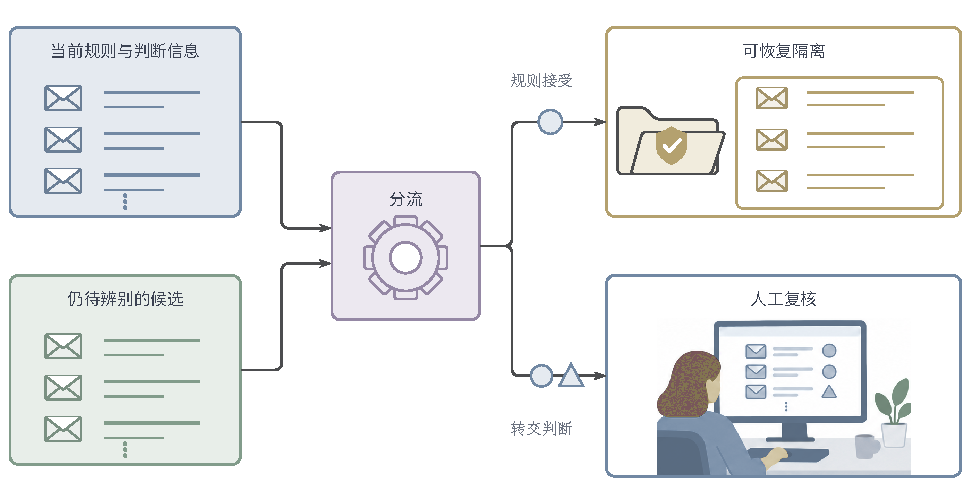
\includegraphics[width=164.600mm]{figures/03-foundations/03-trustworthiness/tikz/reliability-review/figure.pdf}
  \caption{邮件按当前规则的判断依据进入自动隔离或复核。规则接受的判断进入可恢复隔离，仍待辨别的候选转人工接管。分流尚未证明可靠，人工也未假定无误；图~\ref{fig:trust-selective-risk-coverage}继续按处理比例和接受风险计数。}
  \label{fig:trust-reliability-review}
\end{figure*}

\section{不确定性的来源与估计}
\label{sec:reliability-uncertainty}

不同的使用方式需要不同形式的不确定性表达。邮件系统可能要求概率具有频率含义（以便按代价设阈值），可能要求一个预测\emph{范围}以预定比例盖住真实标签（以便高风险时转人工），也可能直接要求自动行动的风险低于某阈值。要满足其中任何一项，前提都是模型能\emph{把“尚未确定”这件事表达出来}。本节先讨论不确定性估计提供了哪些表达；至于这些表达是否正确，要等11.2节用独立数据检验。

“不确定”其实来自两种性质完全不同的原因，区分它们是理解全章的关键。第一种是：即使信息和模型都完美，\emph{同一个输入本身仍可能对应不同结果}，因为决定结果的某些信息（如发件人的真实意图）根本没有出现在输入里。第二种是：固定可观测特征后，我们仍未确定结果的条件规律，有限训练样本不足以区分多种相容的参数或预测分布。知识不足可以和第一种结果随机性同时存在；例如带噪回归既有结果噪声，也可能有未知参数。前者是结果自身的随机波动，后者是我们知识的欠缺；前者再多样本也未必消除，后者增加数据通常能缓解。本节先建立这两类估计对象，11.2节再用独立样本检验它们是否兑现了各自声称的含义。

\subsection{不确定性的来源}
\label{sec:reliability-uncertainty-sources}

设当前观测为$\bm{x}$、真实标签为$y$、训练集为$\mathcal D$。先看第一种不确定性。邮件任务里很容易找到例子：两封文本特征\emph{完全相同}的邮件，一封是正常通知、另一封是钓鱼，因为真正决定类别的“发件人意图”没有写在正文里——仅凭$\bm{x}$，标签本来就不是唯一确定的。这种在\emph{固定观测}之后仍然残留的、结果自身的条件随机性，称为\term{偶然不确定性}（aleatoric uncertainty）。要注意“偶然”不等于“永远无法减少”：如果能拿到新的、能区分意图的信息（如发件账号的历史），这部分随机性是可以下降的；它强调的只是“在\emph{当前已有信息}下结果仍会波动”。

第二种不确定性来自数据量有限。训练样本通过模型形式和学习假设约束候选规律，也会间接限制未见输入处的预测，例如线性模型的同一参数参与所有输入处的计算；但这些约束未必足以区分全部候选，给定模型形式和拟合标准后，往往有\emph{多条不同规律}都与现有数据相容，但它们在数据稀少的区域会给出不同预测。“哪些模型算与数据相容”由具体方法界定，例如贝叶斯方法里后验概率不为零的参数、或集成方法里训练出的各个模型。增加有标签数据通常会缩小这些候选之间的分歧。这种因“知识尚不充分”而产生的不确定性，称为\term{认知不确定性}（epistemic uncertainty）。需要强调，单个模型的一次预测分数\emph{无法}把这两种来源干净地拆开；任何拆分都相对于“我们假定能观察到什么”和“模型族如何设定”而言。

两类不确定性要靠\emph{不同的补充信息}降低，这也是必须区分它们的实际原因。对“相同文本、不同意图”的偶然不确定性，单纯增加同类邮件帮助不大，需要增加能区分意图的\emph{新特征}（如发件域年龄、收件人是否被冒用）；对“某种语言样本太少”的认知不确定性，增加该语言的\emph{有标签邮件}通常就能约束候选规律。因此前者要表达的是“给定现有信息后结果的分布”，后者要表达的是“我们对底层规律有多大把握”，下面两小节的估计方法正是按这两个不同用途设计的。

还要避免一种过度解读：把不确定性分成两类，并不意味着两类的\emph{真实大小}就自动已知了。真实条件分布通常是未知的，模型也可能遗漏了关键因素；无论是参数后验、模型集成还是直接学习条件分布，得到的都只是\emph{在一组假设下}对不确定性的估计。估计手段本身的近似误差（模型族设错、积分没算准等）应当与“被估计的那种不确定性”\emph{分开}报告——“模型很确信”和“模型确实正确”是两回事。

图~\ref{fig:trust-uncertainty-sources}在同一个邮件任务里并排展示两种缺口：左边是特征相同但意图不同（需要表达结果分布），右边是该类样本稀少、三个候选模型给出0.2、0.5、0.8三种预测（需要表达知识不足）。图中数值只是示意分歧的构造概率，不是实测或真实后验。读图时可以验证一个关键判断：在模型和观测假设适当时，增加有信息的同类样本通常有助于减少右侧候选之间的分歧，但不保证每次新增样本都单调减小分歧。但增加这类样本仍无法补上左侧那种“输入里本来就没有意图信息”的缺口。

\begin{figure*}[htbp]
  \centering
  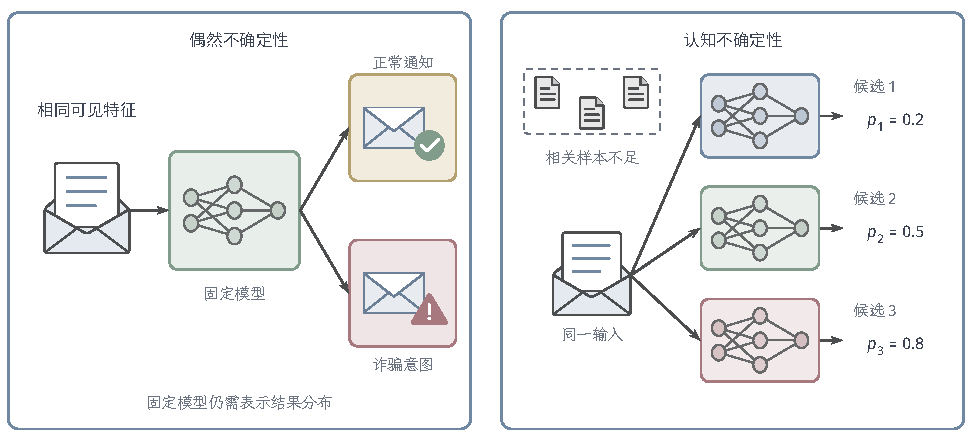
\includegraphics[width=164.600mm]{figures/03-foundations/03-trustworthiness/tikz/uncertainty-sources/figure.pdf}
  \caption{固定观测后比较两类缺口：左侧相同特征对应通知或诈骗意图，模型需表达结果分布；右侧相关样本少，三个候选预测不同，$p_m$表示$p_m(y=1\mid\bm x)$。0.2、0.5、0.8是示意分歧的构造概率，并非实测或后验抽样。两类来源都依当前观测及模型假设定义。}
  \label{fig:trust-uncertainty-sources}
\end{figure*}

\subsection{认知不确定性的估计}
\label{sec:reliability-epistemic-estimation}

先讨论怎样估计\emph{认知}不确定性。如果训练后只保留一个最优模型，我们看到的只是“多条相容规律中的一条”，无法知道数据还容许哪些别的规律、它们在新输入上分歧有多大。一个自然的想法是：\emph{保留一组候选模型，让它们对同一输入各自预测，再比较预测的分散程度}。这里比较的对象必须是\emph{输出预测}而不是参数本身——两组相差很大的参数可能计算出几乎相同的函数，因此“参数分散”不等于“预测有分歧”，后者才与使用风险相关。

贝叶斯方法给“哪些候选规律更可信”分配一套概率权重，即参数后验。下面采用给定协变量$\bm{x}$的条件模型，并假设给定参数后，未来目标与训练集$\mathcal D$条件独立（这是能把联合分布拆成似然乘积的关键假设）。记参数为$\bm{\theta}$、后验密度为$p(\bm{\theta}\mid\mathcal D)$。与其只用一组“最优参数”预测，不如对\emph{每一组}参数下的预测按后验概率加权平均，得到后验预测分布
\begin{equation}
 p(y\mid\bm{x},\mathcal D)
 =\int p(y\mid\bm{x},\bm{\theta})
       p(\bm{\theta}\mid\mathcal D)\,\mathrm d\bm{\theta}.
 \label{eq:reliability-posterior-predictive}
\end{equation}
这个积分把两种不确定性\emph{同时}包含了进来：对固定的一组参数，$p(y\mid\bm{x},\bm{\theta})$内部仍有结果的随机波动；而后验积分又在不同参数（即不同候选规律）之间平均。对二阶矩存在的实值目标，可以用概率论中的全方差公式把这两部分显式拆开
\begin{equation}
 \begin{aligned}
 \operatorname{Var}(y\mid\bm{x},\mathcal D)
 ={}&\mathbb E_{\bm{\theta}\mid\mathcal D}
       \operatorname{Var}(y\mid\bm{x},\bm{\theta})\\
 &+\operatorname{Var}_{\bm{\theta}\mid\mathcal D}
       \mathbb E(y\mid\bm{x},\bm{\theta}).
 \end{aligned}
 \label{eq:reliability-variance-decomposition}
\end{equation}
右端第一项是“每个模型自己的条件方差”按后验平均，对应结果自身的偶然波动；第二项是“各模型预测均值”在后验下的方差，对应参数层面的知识不足——模型之间分歧越大，这项越大。要强调这个分解的\emph{成立边界}：它是在我们假定的概率模型内成立的恒等式，并没有证明现实中的不确定因素已被全部涵盖。如果\emph{所有}候选模型都遗漏了同一个关键因素，它们会高度一致地犯同一个错，此时第二项（模型间分歧）很小，系统性偏差却可能很大。这再次说明“模型很一致”不等于“预测可靠”（可参考\BookChapterRef{chap:random-variables}{卷2《数学准备：概率、因果与决策》第1章“随机变量”}）。

后验预测分布在概念上很清楚，但对深度神经网络\emph{计算}起来通常不可行：参数可能上亿，后验是高维空间中的复杂分布，积分没有解析解，网格离散也不现实。如果退而只取后验密度最高的一组参数（最大后验估计），又等于丢掉了其他所有候选规律的贡献，恰好抹掉了想表达的认知不确定性。因此需要在有限计算预算下\emph{近似}地保留这些贡献，下面是两类常用近似。

第一类近似来自变分推断：不直接求复杂后验，而是选一个\emph{容易采样}的分布族$q_{\bm{\phi}}(\bm{\theta})$（如高斯），用可调参数$\bm{\phi}$让它尽量逼近真实后验。直觉上，我们想用$q$代替后验去做那个积分，近似误差用KL散度衡量；直接最小化KL仍含未知的归一化常数，经过变形可以把目标改写成一个\emph{只含似然和先验、可优化}的形式。设$p(\mathcal D\mid\bm{\theta})$为似然、$p(\bm{\theta})$为先验，并要求证据$0<p(\mathcal D)<\infty$、$q_{\bm{\phi}}$对后验绝对连续、KL有限（这些条件保证下面的重写合法），则最小化$q$与后验的KL散度等价于最小化
\begin{equation}
 \mathcal J(\bm{\phi})
 =-\mathbb E_{q_{\bm{\phi}}}\log p(\mathcal D\mid\bm{\theta})
   +\operatorname{KL}\bigl(q_{\bm{\phi}}(\bm{\theta})
                    \,\|\,p(\bm{\theta})\bigr).
 \label{eq:reliability-variational-objective}
\end{equation}
这个目标的两项各有直观作用：第一项（负对数似然）要求$q$分配了权重的参数必须能\emph{解释数据}；第二项KL把$q$往\emph{先验}方向拉，防止它为拟合数据而偏得太远。由$\operatorname{KL}(q_{\bm{\phi}}(\bm{\theta})\|p(\bm{\theta}\mid\mathcal D))=\mathcal J(\bm{\phi})+\log p(\mathcal D)$可知，证据项$\log p(\mathcal D)$与$\bm{\phi}$无关，所以优化$\mathcal J$与最小化KL给出同一个最优$q$（可参考\BookChapterRef{chap:information-theory-and-statistical-geometry}{卷2《数学准备：概率、因果与决策》第2章“概率分布”}）。但用优化代替积分，并\emph{没有}突破近似族本身的表达能力：例如一个单峰高斯$q$无法同时容纳两个相距很远、却都能解释数据的解释；即使优化完美收敛，这种模型错配依然存在。

第二类近似巧妙地复用了训练中已有的随机机制。Gal和Ghahramani指出，在\emph{特定}设定下，训练时使用的dropout可以被解释为一种变分近似；预测时\emph{不关闭}dropout，对同一输入做多次前向传播、每次用不同的随机失活掩码，再把多次预测平均，就近似了后验预测分布，称为\term{蒙特卡洛失活}（Monte Carlo dropout, MC dropout）\scite{gal2016dropout}。它的好处是几乎不改动已有训练流程；但必须注意，这种贝叶斯解释\emph{依赖}特定的近似模型和正则化对应关系，并不是“给任意已有网络打开dropout，输出的波动就自动是正确的后验不确定性”。

若$M$次随机前向分别输出类别分布$p_m(y\mid\bm{x})$，用平均值$\bar p=M^{-1}\sum_m p_m$近似后验预测。增大$M$只降低\emph{既定近似下}的蒙特卡洛采样误差，使平均结果更稳定；它\emph{不会}修复先验设错、似然设错或近似族过于简单带来的系统性偏差。在低延迟服务中还要权衡：重复前向$M$次的计算成本，与直接对不确定请求拒答所减少的损失，哪个更划算。

还可以完全不拟合参数后验，而是\emph{直接训练多个模型}再汇合它们的预测，这就是\term{深度集成}（deep ensembles）。直觉上，用不同随机初始化（并常配合不同小批量顺序）训练出的多个网络，会落到损失曲面上不同的相容解，它们在数据充足处预测趋于一致、在数据稀少处自然产生分歧，把这种分歧保留下来就补入了单个网络看不到的不确定性。Lakshminarayanan等人用独立初始化、\emph{概率评分}训练（让每个成员不只预测均值还预测自己的方差）和集成预测，给出了一个简单且常很强的基线\scite{lakshminarayanan2017ensembles}，其成员还可并行训练。

以回归为例，成员$m$同时输出预测均值$\mu_m(\bm{x})$和它自己估计的方差$v_m(\bm{x})$。集成总方差同样要包含“成员内部波动”和“成员之间分歧”两部分，等权混合后为
\begin{equation}
 \begin{aligned}
 \bar\mu(\bm{x})&=\frac1M\sum_{m=1}^{M}\mu_m(\bm{x}),\\
 \bar v(\bm{x})&=\frac1M\sum_{m=1}^{M}v_m(\bm{x})
  +\frac1M\sum_{m=1}^{M}
       \bigl(\mu_m(\bm{x})-\bar\mu(\bm{x})\bigr)^2.
 \end{aligned}
 \label{eq:reliability-ensemble-variance}
\end{equation}
用一个教学算例看这两项为什么都不能少：两个成员均值分别为0和2、方差都为1，则混合均值为$(0+2)/2=1$；成员内部波动平均为1，成员均值相对混合均值的分歧为$((0-1)^2+(2-1)^2)/2=1$，总方差为$1+1=2$。只平均各方差（得1）会漏掉“两个模型其实预测得不一样”，只算均值分歧（得1）又会漏掉“每个模型自己都认为结果还会在其预测附近波动”。两项合起来才是混合分布的真实方差。

最后要给集成方法也划一条边界：独立初始化只是\emph{训练中的一个随机来源}，它不保证成员在\emph{真实数据}上独立犯错。由于所有成员共享相同的训练数据、相似的架构和损失函数，它们可能形成\emph{共同盲点}——遇到某类全体都没学好的输入时会一致地、自信地犯错，此时集成分歧照样很小。因此无论MC dropout还是深度集成，其输出的不确定性\emph{是否真的可靠}，仍要靠后面的校准检验、拒答效果检验以及在变化条件下的独立测试来确认，不能仅凭“方法名字带贝叶斯/集成”就采信。

\subsection{偶然不确定性的刻画}
\label{sec:reliability-aleatoric-estimation}

11.1.2节通过改变候选模型观察“规律分歧”，刻画的是认知不确定性；本节固定\emph{一个}候选模型，研究在它看来同一输入下结果本身如何波动，即式~\eqref{eq:reliability-variance-decomposition}第一项的偶然不确定性。做法随任务而变：分类问题直接输出各类别的概率分布；回归问题可以学习随输入变化的完整条件分布，或至少学习随输入变化的均值和方差；如果下游只需要一个区间，甚至不必假设完整分布，直接拟合所需的分位点即可。

要让模型自己学出“噪声有多大”，先得有一个把方差也当作输出的学习目标。最简单的做法是假设$y\mid\bm{x}$服从均值$\mu(\bm{x})$、方差$v(\bm{x})>0$的正态分布，并让网络\emph{同时}输出$\mu$和$v$，再最大化似然（等价于最小化负对数似然）。略去与输出无关的常数后，单个样本的损失为
\[
 \frac{(y-\mu(\bm{x}))^2}{2v(\bm{x})}
       +\frac12\log v(\bm{x}).
\]
这个目标隐含一种自动平衡，值得看清：当某个样本残差$(y-\mu)^2$很大时，模型可以通过\emph{增大}$v$让第一项变小（等于承认“这里我本来就拿不准”），但第二项$\tfrac12\log v$会同步增大，对“无谓地把方差调很大”施加惩罚——所以模型不能靠把所有点的方差都推到无穷来逃避拟合。不过正态假设也限定了结果的形状：例如邮件进入人工流程后的处理时长可能呈\emph{双峰}（多数很快、少数被深度调查很久），这时报告一个中间均值加很大方差，未必能为“何时预警超时”提供足够信息，可能需要更灵活的分布或直接预测分位点。

当决策只依赖某个分位点（如“95\%的邮件应在多长时间内处理完”）时，可以完全不假设分布形状，直接学习分位点。对$\tau\in(0,1)$，用残差$u=y-q_\tau(\bm{x})$定义\term{分位数损失}（因图像形似又称弹球损失 pinball loss）：
\[
\rho_\tau(u)=u\bigl(\tau-\mathbb I\{u<0\}\bigr),
 \qquad u=y-q_\tau(\bm{x}).
\]
为什么最小化这个分段线性损失能得到分位点？直观地说，$\tau>1/2$（高分位）时它对“估低了”（$u>0$）罚得更重，于是最优解会\emph{上移}以减少低估；$\tau<1/2$时则对高估罚得更重、最优解下移。当相应期望有限时，最小化真实条件分布下的期望损失，可以得到一个$\tau$分位点$q$，其一般条件为
\[
 \mathbb P(Y<q\mid\bm x)\leq\tau
 \leq\mathbb P(Y\leq q\mid\bm x).
\]
因此不超过$q$的概率至少为$\tau$，不低于$q$的概率至少为$1-\tau$。只有分位点处没有概率原子、条件分布在该处连续时，才能把这两侧写成等号；离散结果在$q$处可能有大量概率质量，不能笼统近似为$\tau$和$1-\tau$。分别用大$\tau$和小$\tau$学上下界，就拼出一个预测区间。当然，有限数据、模型容量和优化误差都可能使实际覆盖偏离名义水平，区间仍需在独立数据上校准。

这里要再次区分“被估计对象”和“估计手段”：网络输出的方差、分位点\emph{本身也是学出来的}，同样会受到数据不足（认知不确定性）的影响，不能把它直接当成真实的偶然不确定性。把多个模型的结果分布混合后，得到的范围会\emph{同时}包含内部波动和候选分歧，因此仍应在未参与拟合的独立样本上检验。还要区分两种区间：\emph{预测区间}保护的是\emph{未来一个具体结果}$y$的落点（因此必须容纳结果噪声），而参数的置信区间或贝叶斯可信区间保护的是\emph{未知参数}；只把参数区间传播出去未必能覆盖未来观测的随机噪声。

生成式模型让“概率”一词的对象发生了变化，需要特别警惕。模型给出一个词元序列$(w_1,\ldots,w_T)$的概率，是各步条件概率的乘积，它衡量的是“模型\emph{生成这段措辞}的倾向有多大”，而\emph{不是}“这段陈述在现实中为真的概率”。同一条事实可以有许多种等价措辞，模型可能给流利的错误表述也打出很高的序列概率。因此评价生成内容前，必须先确定\emph{评价单元}：是单条事实主张、完整答案，还是整个任务的最终结果，再据此选择评分方式。

要检验“会不会给出无依据的事实”，光看模型本体不够，必须\emph{冻结整个生成程序}：模型版本、系统提示、检索到的内容、采样参数、重试次数、结果筛选和核验器，因为它们共同决定最终答案。例如把事件定义为“答案中的每条事实主张都有指定来源支持”，就要事先规定：怎样把文本切成主张、什么样的来源算合格来源、来源之间矛盾时由谁裁决；然后用一批\emph{没有}参与这些设定的评价样本来估计风险。人工或自动评判者自身的漏报、误报属于测量误差，要单独检查。

同一套程序也可以用来检验“语义不确定性”或拒答分数是否真的有用。如果按前面定义的事件（有无合格来源支持）来检验，就应报告：缺少来源支持的主张占多少比例、系统因此自动处理的比例是多少、转人工的成本多高。若还想进一步报告“事实错误率”，则必须\emph{另行}定义“在现实中正确”这一事件、配套事实核验标准并测量评判误差——“有来源支持”和“现实中正确”是两件事（来源本身可能出错），不能互相代替。这样才真正回应了章首的生成问题：低词元熵、语义上高度一致或评判模型给高分，都只是\emph{代理信号}，必须通过对应的\emph{事实事件}核验，不能直接等同于内容正确。

\section{可靠性的检验}
\label{sec:reliability-evaluation}

11.1节解决了“怎样\emph{产出}概率、区间和分歧分数”，但任何模型都能输出看起来很自信的数字，所以接下来必须用\emph{独立}于训练和调参的真实结果来检验这些输出是否兑现含义。第一步检验\emph{数值本身}：所有被报告为0.9的事件，在总体里是否真的约有九成发生（校准）。

第二步检验一个\emph{不同}的能力：即使数值不精确，分数能否\emph{识别出哪些输入更容易出错}？只有当模型能把高损失的预测排到“不确定”的一端，拒答机制才可能通过放弃这些输入来降低自动处理的风险。这种“风险排序”能力与“概率数值准确”是两回事，要分别评价。

第三步是\emph{局部}检验：前两步若只在全体上取平均，某个语言或某类设备上的较差表现可能被其他群体的好结果平均掉。因此要在声明的使用范围内，对重要子群体\emph{重新计算}校准、覆盖和选择风险，看清证据\emph{对谁}成立。这一步只是给已有指标加上条件，而不是另造一个综合分数。

所有这些检验都必须在模型训练、概率修正和阈值选择\emph{全部结束之后}，用独立数据一次性完成；如果反复看测试结果再回去调模型或阈值，测试集就重新参与了开发，独立性被破坏、结论会偏乐观。生成任务还要额外固定事件定义、评判者和采样方式，并区分“来源存在”“来源支持该主张”“主张在现实中正确”三个层次，字符串匹配代替不了这些判断。诊断性分析可以展示样本间的差异，但要下“达标”结论仍需明确抽样条件并报告估计误差。

\subsection{概率与预测范围的检验}
\label{sec:reliability-output-evaluation}

先界定校准检验\emph{不能}涵盖的一面，避免把覆盖率当作唯一追求。一个模型可以给出很窄、很“自信”的预测范围，却把范围\emph{整体放错}了位置（真实值几乎从不落入）；反过来，如果把分类集合直接取成所有类别、把回归区间取成$(-\infty,\infty)$，覆盖率当然是100\%，却对选行动毫无帮助。因此除了检查是否覆盖，还必须按用途评价范围提供的\emph{信息量}（平均大小、长度）。不过要澄清：当承诺只是“边际覆盖率”时，范围大小影响的是\emph{效率}，并不是覆盖成立的前提——一个很宽的集合完全可以既有效又没用。

回到章首的问题：“0.9”应该对照什么来检验？在二分类中记$y\in\{0,1\}$，用$p(\bm{x})$表示模型报告的$y=1$概率。校准要检验的是：在所有\emph{报告了相同概率}的输入里，事件发生的平均频率是否等于该概率，即
\begin{equation}
 \mathbb E[y\mid p(\bm{x})]=p(\bm{x})
\quad\text{相对于当前联合分布几乎必然成立},
 \label{eq:reliability-calibration}
\end{equation}
\term{校准}（calibration）因此被定义为：相同（或近似相同）的概率报告，在总体中对应相符的长期事件频率。写成条件期望的形式$\mathbb E[y\mid p(\bm{x})]=p(\bm{x})$还能直接用于连续分数，避免了“精确等于某个连续概率值的样本可能一条都没有、无法计算普通频率”的技术困难。

这里藏着一个反直觉但极重要的事实：\emph{校准很容易达到，即使模型完全不看输入}。如果垃圾邮件在总体中占10\%，模型对\emph{每一封}邮件都恒常报告0.1，那么“报告0.1的邮件中确有10\%是垃圾邮件”严格成立——它是校准的，但它对具体邮件毫无区分能力，无法用于筛选高风险邮件。因此“概率数值准确（校准）”和“能否区分不同风险（区分能力）”是两个独立的要求，要分别评价；平均覆盖率、个体层面的信息量、行动损失也不能互相代替。Guo等人的实证研究同样发现，神经网络分类准确率的提高并不自动带来良好的概率校准，常常反而更过度自信\scite{guo2017calibration}。

图~\ref{fig:trust-calibration-discrimination}把这一点画得很直观：左图比较理想校准关系与过度自信关系；右图构造两个频率为20\%和80\%的等大群体——恒常报告0.5在总体上是校准的，而分别报告0.2和0.8也\emph{同样}校准，但只有后者真正区分了高风险和低风险群体。

\begin{figure*}[htbp]
  \centering
  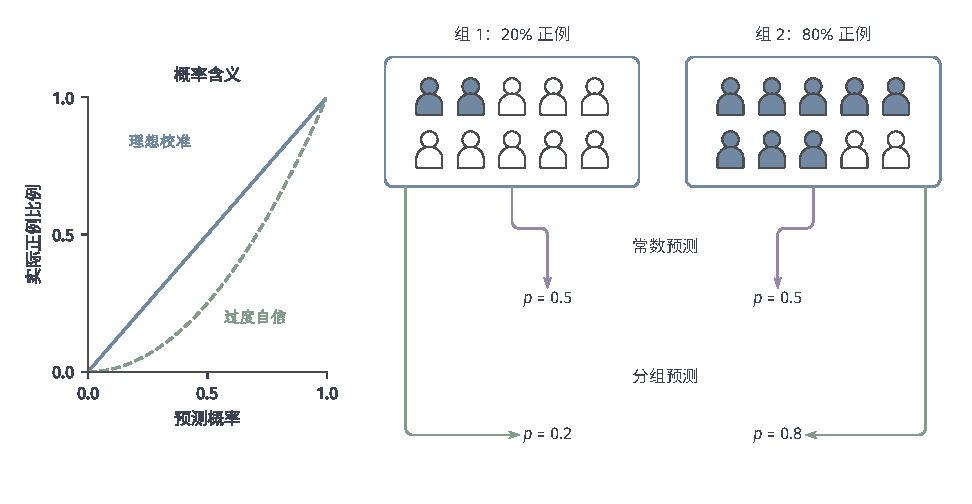
\includegraphics[width=164.600mm]{figures/03-foundations/03-trustworthiness/tikz/trust-calibration-discrimination/figure.pdf}
  \caption{左侧用实线理想关系和虚线过度自信关系示意校准，两者均非实验。右侧构造等大群体，事件频率20\%和80\%；常数0.5总体校准，分组0.2与0.8也校准，后者同时提供组间区分。}
  \label{fig:trust-calibration-discrimination}
\end{figure*}

\paragraph{概率校准的经验修正}

如果模型的\emph{类别决策}已经满足要求，但独立校准数据暴露出它的概率\emph{系统性偏大}（过度自信），可以在不重新训练分类器的情况下，只修正最外层的概率表达。最简单的温度缩放（temperature scaling）只用一个正参数$t>0$去缩放未归一化的类别对数分数（logit）$z_k(\bm{x})$，然后重新归一化：
\[
 p_t(y=k\mid\bm{x})
 =\frac{\exp(z_k(\bm{x})/t)}
        {\sum_j\exp(z_j(\bm{x})/t)}.
\]
参数$t$在一份\emph{独立校准集}上用负对数损失选择。由于softmax对全体logit统一缩放，正温度\emph{不会改变各类别的相对排序}、也不会改变argmax类别，所以不影响分类决策本身，只改变概率分布的\emph{集中程度}；但下游若用固定概率阈值来隔离或拒答，这些行动仍会因概率数值改变而变化，必须按第~\ref{sec:trust-context}节的损失关系重新检查。还要注意，校准集上的修正只是经验调整，并不自动带来任何关于新分布的形式保证。

参数方向很直观：$t>1$把logit差距缩小、使概率分布趋于平缓，用于纠正过度自信；$0<t<1$拉大差距、使分布更集中，用于纠正不自信。只用一个参数的好处是小样本下也能稳健估计，代价是能修正的偏差类型有限——当不同类别各自的偏差方向不同时，单一温度可能不够，可换用类别相关的仿射变换或单调映射，但这些方法参数更多、小样本估计更难，甚至可能改变分类决策边界；复杂度该选多大，仍要在独立数据上检验，校准集上的拟合损失本身不能决定。

修正之后要针对\emph{输出承诺的内容}重新检验：概率输出就拿报告概率对照事件频率、对整份分布打分；集合或区间输出就对照名义覆盖率、同时报告宽度。这些检验确认的是输出数值的含义；而“输出能否用来筛选输入、拒答能否降低损失”是下一小节的决策问题，两者不能混为一谈。

连续概率在有限样本里无法逐值观察频率，实践中把概率轴\emph{预先}切成若干区间（bin），画成可靠性图：对非空区间$b$，记其中样本数$n_b$、平均预测$\bar p_b$、实际正例比例$\bar y_b$，用二者绝对差按样本占比加权，得到期望校准误差的估计
\begin{equation}
 \widehat{\operatorname{ECE}}
 =\sum_{b=1}^{B}\frac{n_b}{n}
       |\bar p_b-\bar y_b|.
 \label{eq:reliability-ece}
\end{equation}
其中$B$是区间数、$n$是总样本数。分箱口径会显著影响数值：箱太粗会把“先高估、后低估”的相反偏差在一个箱内抵消，箱太细则每箱样本少、频率本身波动剧烈。因此ECE必须连同\emph{分箱方式和每箱样本量}一起报告，用不同分箱得到的ECE不能直接比较大小。

除了分箱诊断，还可以用\emph{严格适当评分规则（真实分布是期望评分损失的唯一最优报告）}直接给整份概率打分，常用的是负对数损失和Brier分数；二分类Brier经验分数为$n^{-1}\sum_i(p(\bm{x}_i)-y_i)^2$。为看清它为什么能奖励“说真话”，固定一个输入、记其真实条件概率为$\eta(\bm{x})$，对期望平方误差展开：
\[
 \mathbb E[(p-y)^2\mid\bm{x}]
 =(p-\eta)^2+\eta(1-\eta).
\]
右端第二项$\eta(1-\eta)$与报告值$p$无关（是该输入不可消除的噪声），与$p$有关的只有$(p-\eta)^2\geq0$，因此期望Brier分数恰好在\emph{如实报告$p=\eta$}时最小。不过在\emph{有限样本}上算出的总分同时受校准和区分能力影响，不能用一个总分替代分箱的校准诊断。

凡是“如实报告真实分布时期望损失最小”的评分，统称\term{适当评分规则}（proper scoring rule）；最优解唯一时称\emph{严格}适当。负对数损失也有这种性质：其期望等于真实分布的熵加上真实分布到报告分布的KL散度，因此把一个实际会发生的事件报告成极不可能，会受到很重的惩罚。两者风格不同：Brier分数有界、对极端错误的惩罚相对温和，负对数损失对“自信地答错”惩罚极重。但无论哪种，它们评价的都是\emph{概率质量}，并不等于“误拦一封重要邮件”的实际行动损失——后者仍要按第10章的行动损失另行计算。

多分类问题里“校准”有强弱不同的几种含义，必须事先声明要求的是哪一种：只比较最大概率与正确率，检验的仅是top-1预测；逐类比较每一类的报告概率与该类出现频率，检验每个类别的一维校准；最严格的\emph{完整向量校准}要求“报告同一概率向量的样本里，各类别出现的比例都等于向量分量”。越严格要求的数据量越大。只看最高分会漏掉其余类别上的偏差，而这些偏差可能影响代价敏感决策和共形集合的构造。

可靠性图还必须显示每个区间的\emph{样本量}，否则一个比例数字可能看起来很精确、其实只由极少数样本支撑。例如某箱只有10封邮件、平均报告0.9、其中9封是垃圾邮件（9/10），这与“真实概率就是0.9”相去甚远——二项波动很大。正确做法是预先固定分箱、补充数据、并为每箱报告二项置信区间，把9/10背后的估计不确定性显示出来。反过来，看到结果后再反复合并或拆分箱子去凑一条好看的对角线，会改变评价过程本身，得到的“校准”是虚假的。

对预测集合$C(\bm{x})$，覆盖率用指示函数$\mathbf 1\{y\in C(\bm{x})\}$的样本均值估计，同时必须报告集合的平均大小（回归则报告区间平均长度），否则无法判断覆盖是不是靠“无脑取全集”得到的。一批样本达到90\%覆盖，只是对“90\%覆盖”这一承诺的\emph{经验}支持，仍含抽样误差；即便总体覆盖率达标，也不代表每个群体、每一类输入都达标，局部覆盖要按11.2.3另行检验。

\begin{example}[校准与区分能力]
\label{ex:reliability-constant-score}
构造一个正例比例10\%的总体。甲始终报告0.1，在总体上校准；乙把样本分成占比$5/6$和$1/6$的两组，各报告与组内频率相符的0.02和0.5。两组总正例比例为$(5/6)\times0.02+(1/6)\times0.5=0.1$，所以乙也校准，却区分了风险。若要筛选高风险输入，我们还需评价这项区分，校准误差小本身无法完成选择。
\end{example}

\subsection{风险识别与拒答效果的检验}
\label{sec:reliability-selection-evaluation}

校准回答“概率数值准不准”，但很多系统真正用不确定性做的事是\emph{拒答}：对拿不准的输入不做自动决定、转人工处理。这里要检验的是另一种能力。先注意一个反直觉点：一个\emph{未校准}的分数仍可能很好地\emph{排序}风险（把错误预测排到高不确定端），从而支持有效的拒答；反过来，恒常报告总体正例率的模型虽校准，却完全无法区分该拒哪些。\term{选择性预测}（selective prediction）就是允许系统拒答、只对\emph{一部分}输入做自动处理的框架；评价时必须\emph{同时}报告两件事：被接受（自动处理）部分的风险，以及被放弃的自动处理量——只报一个都会误导。

用数学把这两个量分清。记接受函数$g(\bm{x})\in\{0,1\}$（1表示自动处理）、单次预测损失为$\ell(f(\bm{x}),y)$。\emph{接受比例}以\emph{全部请求}为分母，\emph{接受风险}则只在\emph{被接受}的请求上平均：
\begin{equation}
 \begin{aligned}
 c(g)&=\mathbb P(g(\bm{x})=1),\\
 R_{\mathrm{sel}}(f,g)
 &=\frac{\mathbb E[\ell(f(\bm{x}),y)g(\bm{x})]}
         {c(g)},\qquad c(g)>0.
 \end{aligned}
 \label{eq:reliability-selective-risk}
\end{equation}
在独立测试中，用一个不确定性分数$u(\bm{x})$（越大越不确定）按阈值$t$构造接受规则$g_t(\bm{x})=\mathbb I\{u(\bm{x})\leq t\}$：分数不超过$t$才自动处理。记录每条样本的分数、预测和标签后，分别用样本估计接受比例和接受风险：
\begin{equation}
 \begin{aligned}
 \hat c(t)&=\frac1n\sum_{i=1}^{n}g_t(\bm{x}_i),\\
 \hat R_{\mathrm{sel}}(t)
 &=\frac{\sum_{i=1}^{n}\ell(f(\bm{x}_i),y_i)g_t(\bm{x}_i)}
          {\sum_{i=1}^{n}g_t(\bm{x}_i)}.
 \end{aligned}
 \label{eq:reliability-empirical-selective-risk}
\end{equation}
当没有任何样本被接受时分母为零、风险无定义，报告时要排除或注明这一点。让阈值$t$从松到紧变化，就得到一条$(\hat c(t),\hat R_{\mathrm{sel}}(t))$的\emph{风险—处理比例曲线}：在\emph{相同接受比例}下接受风险越低，说明分数在这批测试中越成功地把高损失输入留在了拒答端。用\emph{随机拒答}作为基准很重要——随机丢掉一部分输入不会改变留下部分的期望错误率，因此只有明显优于随机拒答，才能说分数真的识别了风险，而不只是单纯减少了工作量。

\begin{example}[相同拒答比例下的不同效果]
\label{ex:reliability-risk-ranking}
构造十封测试邮件，其中两封分错，损失取零一值。甲把两封错误排为最不确定，拒绝后八封均正确，经验风险0；乙拒绝的却是两封正确邮件，八封中仍错两封，风险$2/8=25\%$，比全处理的20\%高。随机拒绝两封，留下部分的期望错误率仍20\%。拒答量相同，收益因排序而异，这项比较没有检验分数的概率校准。
\end{example}

图~\ref{fig:trust-selective-risk-coverage}把同十封邮件按两种分数排序。接受区域的编号给出式~\eqref{eq:reliability-empirical-selective-risk}的分母，错误计数给出分子。两者都接受八封，风险不同，说明减少处理量只有在筛选出高损失输入时才降低当前接受风险。

\begin{figure*}[!htb]
  \centering
  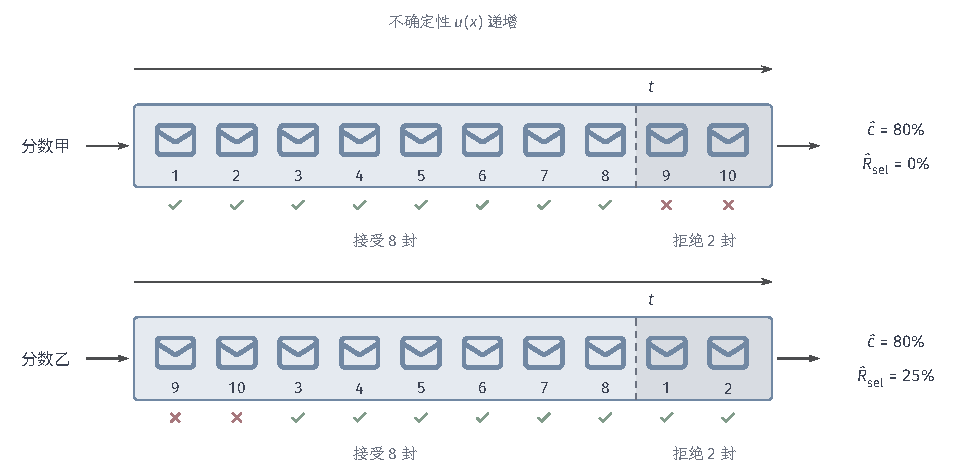
\includegraphics[width=164.600mm]{figures/03-foundations/03-trustworthiness/tikz/trust-selective-risk-coverage/figure.pdf}
  \caption{按示例~\ref{ex:reliability-risk-ranking}将十封邮件依不确定性递增排列，9、10号的$\times$为错误，其余$\checkmark$为正确。蓝区接受八封、灰区拒绝两封。$\hat c(t)$以全部为分母估计$c(g_t)$，$\hat R_{\mathrm{sel}}(t)$以接受数为分母估计$R_{\mathrm{sel}}(f,g_t)$；经验零风险仍未保证总体零风险。}
  \label{fig:trust-selective-risk-coverage}
\end{figure*}

风险—处理曲线是在一批测试上扫出所有阈值得到的\emph{诊断工具}，真正部署只会选其中一个工作点，因此阈值要先用\emph{验证集}确定并冻结，再在\emph{另一份独立测试集}上报告该点的接受数、接受风险及其置信区间。这里有两个易犯的错误：其一，接受数很少时（只自动处理最有把握的少数几封），即使零错误也无法把总体接受风险压得很小——10封里对10封，95\%上界仍很宽；其二，直接在测试曲线上挑“最好看”的点再报告其风险，等于又让测试集参与了选择，会得到偏乐观的数字。

图~\ref{fig:trust-risk-coverage-curve}在示例~\ref{ex:reliability-risk-ranking}的完整排序上，依次计算只接受最有把握的1封、2封……直到10封时的风险：甲到第9封才纳入第一个错误，乙第1封就接纳了错误；当全部处理时两者都回到2/10。这条曲线的具体形状完全取决于排序质量，不能想当然地认为“阈值越紧风险一定单调下降”——若排序把正确邮件误判为不确定，反而可能越拒越糟。

\begin{figure}[!htb]
  \centering
  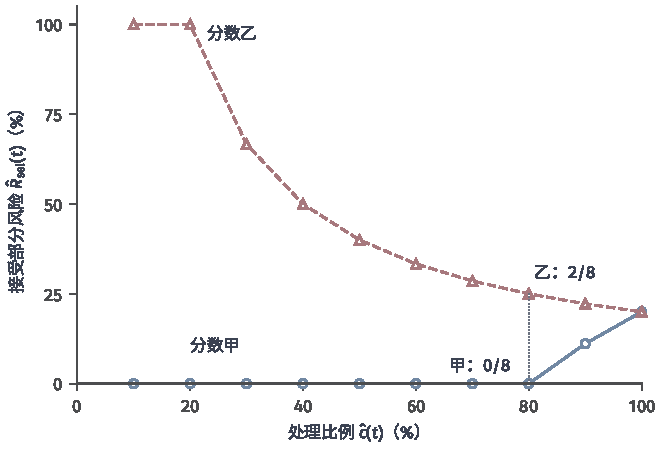
\includegraphics[width=\linewidth]{figures/03-foundations/03-trustworthiness/matplotlib/trust-risk-coverage-curve/figure.pdf}
  \caption{在图~\ref{fig:trust-selective-risk-coverage}完整排序上依次接受1至10封，空心圆为甲、虚线三角为乙。80\%处理时风险0与25\%，全部处理都20\%。点为教学计数的精确比值，无测量误差；零接受时风险无定义，未画对应点。}
  \label{fig:trust-risk-coverage-curve}
\end{figure}

实践中最常见的接受规则是“最大类别概率超过某阈值才自动处理”，但要明白它\emph{只在特定损失设定下}才直接对应风险最小化。当误拦远比漏放昂贵时，接受规则必须把类别概率\emph{和两类错误的代价}一起放进来——同样是0.9的垃圾邮件概率，在“仅提醒人工核查”和“直接永久删除”两种用法下，能否自动处理的答案可能完全不同。

为看清这一点，推导理想的接受规则。设对输入$\bm{x}$自动预测的条件期望损失为$r(\bm{x})$，转人工复核被理想化为一个固定成本$c_{\mathrm r}$（假设人工不会再错）。与第10章示例~\ref{ex:trust-review-cost}一样逐输入比较两者：当$r(\bm{x})\leq c_{\mathrm r}$时自动处理更划算，否则转人工。只有在\emph{零一损失、真实类别概率已知、且自动处理时总是选最大概率类别}这三个条件同时成立时，才有$r(\bm{x})=1-\max_k p(y=k\mid\bm{x})$，此时“最大概率阈值”才是最优规则。若人工也会犯错、或复核队列拥堵，复核成本还会随输入和系统负载变化，简单阈值便不再最优。

接受风险和“全体错误率”使用不同分母，二者数值可能相差很大，务必分清。例如100个请求只接受10个、其中错1个：以接受数为分母的接受风险是1/10=10\%，但以全部请求为分母的“接受且错误”比例只有1/100=1\%。降低处理量天然会压低后者，但\emph{不能}据此声称前者（我们承诺的接受风险）已达标。完整核算还要计入人工复核的错误率和延迟；这两个分母一个都不能在报告中省略。

\subsection{局部条件下的检验}
\label{sec:reliability-conditional-evaluation}

总体平均可能掩盖局部问题：在声明的使用范围内，某种语言上的高错误率完全可能被其他语言的好结果在平均后藏起来。局部检验保持\emph{使用范围不变}，按事先认定的重要子群体（语言、设备、时间段、任务类型等）\emph{重新计算}校准、覆盖和选择风险，以确定总体证据究竟对\emph{哪些人、哪些条件}成立。这里保持系统声明的使用范围不变，但把评价分布条件化到各个子群：总体风险对整个声明总体平均，组内风险对相应条件分布平均，分母与条件已经改变，组内数字不能继续解释为原总体平均。

切片应由\emph{使用要求事先设定}，而不是看完数据再挑最差的组。记组$S$中的样本索引为$I_S$、样本数$n_S=|I_S|>0$，则该组的集合覆盖率只在组内取均值：
\begin{equation}
 \widehat{\operatorname{Cov}}_S
 =\frac1{n_S}\sum_{i\in I_S}
   \mathbb I\{y_i\in C(\bm{x}_i)\}.
 \label{eq:reliability-group-coverage}
\end{equation}
在组内比较时，要\emph{同时}保存样本数、区间长度（或集合大小）和覆盖率的\emph{置信区间}，否则一个点估计没有意义。组内校准要在该组重新比较报告概率与事件频率；组内拒答要重算该组的接受比例与接受风险，其风险分母是\emph{该组被接受的样本数}；若某组没有任何样本被接受，就无法对该组的自动处理风险给出直接经验估计。

一个教学算例说明总体达标不等于各组达标：1000封邮件中常用语言900封、少见语言100封，集合分别覆盖846和54封。总体覆盖率是$(846+54)/1000=90\%$，看起来恰好达标，但拆开看常用语言是$846/900=94\%$、少见语言只有$54/100=54\%$。若承诺的是“\emph{每种}语言都达到90\%”，总体90\%根本没有验证这条承诺，还必须在各组内估计误差。校准图和拒答曲线同理，都可能被总体平均掩盖。

切片越小，估计的随机波动越大，解读时要克制：某组的置信区间若仍包含不达标的值，只能说“证据\emph{尚不足以}确认达标”，而不能反过来说它不达标；两组点估计接近也不能确认它们相同。若在大量切片里专门挑表现最差的，那个极值很可能只是随机波动。正确纪律与第10章一致：看到异常后\emph{事后}选定的切片只能用于诊断，要据以下结论必须换用新数据确认、或使用多重比较校正；即使所有事先指定的有限组都检验了，也仍然不代表对每一个\emph{具体输入}都有保证。

还要划清局部检验与下一章鲁棒性的界限：切片检验只是在\emph{原声明总体内部}细分；如果时间、来源、设备或扰动已经使数据进入一个\emph{新范围}（训练时的分布关系不再成立），那就不是条件化能解决的，需要重新声明变化的性质和任务语义，并重新建立证据。下一章将研究这种分布变化，以及变化后预测、不确定性表达和拒答机制是否会\emph{一起}失效。

小结11.2节：如果一条主张同时涉及概率解释、风险排序和重要局部条件，就需要校准、风险—处理曲线和局部复测\emph{三类证据共同}支持；若只承诺其中一项，则只选择对应的事件检验（数值、筛选效率或条件损失）。复合承诺中某一项失败，恰好指出了对应的能力缺口；即使三项都达标，结论也只在声明的数据范围和估计误差内成立，不能升级为“对任意未来输入都可靠”的保证。

\section{可靠性的保证}
\label{sec:reliability-guarantee}

11.2节是\emph{事后检验}一个已经训练好的模型；本节更进一步，讨论怎样\emph{主动构造}出在明确条件下\emph{保证}满足要求的程序。构造分两支，对应两类不同事件。第一支是\emph{预测范围覆盖}：保证真实答案以预定概率落入我们给出的集合或区间，其中既包括对可交换样本的一次预测，也包括部署中持续获得标签时的长期覆盖频率。第二支是\emph{决策程序风险}：直接约束“预测+接受规则+拒答”这套完整程序的行动损失。由于覆盖事件（答案在不在集合里）和风险事件（行动造成多大损失）根本不同，这两类保证不能互相替代或推出。

\subsection{保证对象与成立条件}

给出任何保证之前，先要把五件事连同概率空间写清楚：\emph{随机事件}是什么（结果进入集合，还是自动行动产生损失）、\emph{目标水平}（覆盖率$1-\alpha$还是风险上限）、\emph{总体}、\emph{时间范围}（一次预测还是长期序列）、以及数据之间满足什么关系。随机性可能来自校准样本和新样本的抽取、验证集的抽取、或在线反馈。还要牢记覆盖承诺\emph{不}保证集合足够小（取全集平凡地覆盖），从集合里任取一个答案也未必正确；接受风险下降也不代表包含人工成本的\emph{全部请求}总成本下降。

这些保证的成立，靠的是数据取得方式和流程\emph{实际满足}某种关系——独立同分布、可交换、或在线反馈可被观察——而\emph{不是}靠模型把训练损失降得足够低：即使训练误差为零，若校准样本与未来样本不满足可交换性，也不能直接用本节定理宣称共形覆盖。实际覆盖仍可能达标，但需要另外的依据；原定理不能使用不等于覆盖必然失败。下面三个小节正是沿三种不同机制构造保证：共形预测利用\emph{校准秩}在可交换性下推出覆盖；集中不等式利用\emph{经验损失}在独立同分布下控制总体风险；在线方法利用\emph{误差反馈}控制长期频率。

保证的\emph{强度}还由量词（概率平均在谁身上）决定，必须在报告时逐层写明随机对象，三者不可混用。\emph{边际覆盖}同时对校准样本和新样本取平均，它允许少数“运气差的整批校准样本”产生较宽或较差的集合；\emph{期望风险}对未来样本平均损失；而\emph{高概率风险保证}则要求：以至少$1-\delta$的概率（$\delta$是事先设定的验证失败概率上限），由随机验证集选出的程序其总体风险不超限——它额外排除了“抽到一批特别不巧的验证数据”这种情况，通常要付出更多样本或更保守的选择。

\subsection{预测范围的覆盖保证}

\paragraph{可交换数据下的边际覆盖}

先解决“怎样在\emph{不}要求模型概率校准的前提下，给出一个有覆盖率保证的集合”。直观出发点是：先有一个衡量“候选答案$y$与模型对输入$\bm{x}$的预测有多不符”的评分$s(\bm{x},y)$（分数越大越不符），再用一批\emph{校准样本}的分数分布来确定“多不符还算可接受”的阈值，使真实答案在新输入上落入集合的频率受控。这就是\term{共形预测}（conformal prediction）。关键在于：\emph{训练好的模型只负责提供分数，覆盖保证完全来自数据的可交换关系和秩的均匀性，与模型自身的概率是否校准无关}\scite{angelopoulos2022conformal}。

务必区分本章出现的两种“校准”：\emph{概率校准}让报告概率与事件频率匹配；\emph{共形校准}只是借用一批校准样本来\emph{选集合阈值}，它不检查概率数值。因此两者可以各自成败：一个概率不准（过度自信）的模型，经共形处理后仍可能得到\emph{有效但很宽}的集合；反过来，一个概率质量很好的模型，如果校准样本与未来样本不满足可交换关系，这里的共形覆盖定理仍不能直接套用。判断时要回到各自的事件。

下面给出去掉随机性后最容易理解的\emph{分裂共形}构造。先用一部分数据训练模型、固定评分函数$s(\bm{x},y)$（大值表示候选答案与模型越不相符），训练集与校准集严格分开。假设在给定训练数据（及训练随机性）后，$n$个校准样本和一个未来样本\emph{可交换}——直观说，这$n+1$个样本地位对称、没有哪一个特殊——并且对它们使用\emph{同一个固定}评分。对校准样本算出$s_i=s(\bm{x}_i,y_i)$。给定目标错误水平$\alpha$，用秩确定接受阈值和集合：
\begin{equation}
 k=\lceil(n+1)(1-\alpha)\rceil,\qquad
 C_\alpha(\bm{x})=\{y:s(\bm{x},y)\leq q\},
 \label{eq:reliability-conformal-set}
\end{equation}
当$k\leq n$时，取校准分数从小到大排列后的第$k$个（顺序统计量）作为阈值$q$；当$k=n+1$时没有足够大的校准分位数可取，令$q=+\infty$（集合包含全部标签）。最后这种情况说明共形的一个底线：当要求的覆盖率高到样本量支撑不起一个非平凡阈值时，它宁可给全集以\emph{保持有效}——但此时集合失去了区分信息，下游要警惕。

覆盖为什么成立？先考虑分数无并列的情形。给定训练部分后，可交换性使未来分数在全部$n+1$个分数中的升序秩均匀。$k\leq n$时，校准分数的第$k$\emph{小}值作为阈值；未来秩不超过$k$便保证未来分数不超过该阈值，所以覆盖概率至少为$k/(n+1)\geq1-\alpha$。$k=n+1$时按约定取全集，覆盖直接成立。有并列时，普通确定排名不再均匀，可以先附加独立随机数打破并列作秩论证；实际程序将全部等于阈值的分数纳入，不会比随机打破并列的构造更少覆盖，因此仍有保守的“至少”保证：
\[
 \mathbb P\bigl(y_{n+1}\in C_\alpha(\bm{x}_{n+1})\bigr)
 \geq1-\alpha.
\]
要看清这个概率的量词：即使条件于训练样本和训练随机性，它仍然是\emph{同时}对校准样本和未来样本的抽取取平均的；解除训练条件后不等式也成立。用“$\leq q$”把并列分数一并纳入只会增大集合、不减覆盖。\emph{在覆盖目标固定之后}，真正要下功夫比较的是评分函数——它决定了集合通常多小、对下游行动多有用。

评分的选择只影响集合的\emph{形状和宽度}，不影响上面的边际覆盖逻辑。回归取绝对残差$s=|y-f(\bm{x})|$，集合就是对称区间$[f(\bm{x})-q,f(\bm{x})+q]$；分类可取$s(\bm{x},y)=1-p(y\mid\bm{x})$，保留模型概率不小于$1-q$的类别。比较两个评分器时，应固定覆盖目标，在独立数据上比较平均区间长度或平均集合大小；非对称代价的任务还要再比较行动损失。

必须如实说明边际定理的\emph{边界}：它\emph{没有}承诺“对每一个具体输入$\bm{x}$覆盖率都是$1-\alpha$”（条件覆盖），也\emph{没有}承诺“对某一批\emph{固定}的校准样本算出的集合恰好覆盖”——这两者都比边际保证强。要对某子群体保证，需要该群体内有足够样本且满足相应可交换关系；要在变化环境下保证，需要新的假设或在线方法。因此“分布无关（distribution-free）”指的是\emph{不限制误差分布形状}，绝\emph{不}等于“没有任何抽样条件”。

图~\ref{fig:trust-conformal-construction}按顺序展示整个构造：先在独立数据上训练并固定评分，再把校准残差排序选阈值，最后套到新输入上形成范围。图中教学残差$0.1,0.2,\ldots,0.9$，取$n=9,\alpha=0.2$得$k=8,q=0.8$。读图注意：真正承担覆盖论证的是\emph{可交换性}，图中的具体宽度只用于说明构造，不能当作覆盖率的实测证据。

\begin{figure*}[htbp]
  \centering
  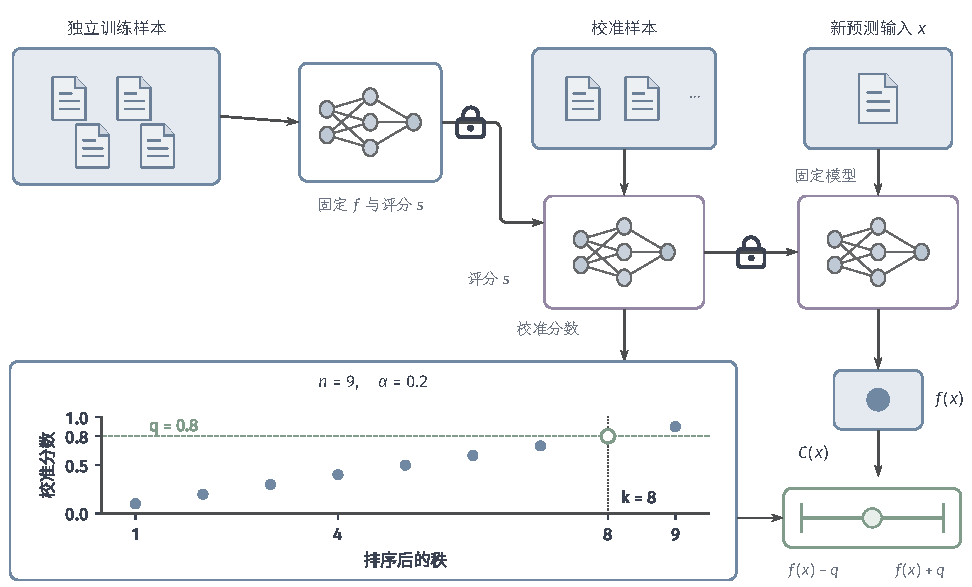
\includegraphics[width=164.600mm]{figures/03-foundations/03-trustworthiness/tikz/trust-conformal-construction/figure.pdf}
  \caption{独立训练先确定评分，再由校准秩选择集合阈值。教学残差$0.1,0.2,\ldots,0.9$取$n=9,\alpha=0.2$，于是$k=8,q=0.8$；绝对残差给右侧区间。图解释排序和构造，没有测量覆盖率。}
  \label{fig:trust-conformal-construction}
\end{figure*}

\paragraph{自适应范围与条件覆盖边界}

边际共形只保证“平均意义的覆盖”，留下两个自然的改进方向，要分开问。其一，区间宽度能否\emph{随输入难度调整}——对本身很确定的输入给窄区间、对噪声大的给宽区间——以提高信息量？其二，覆盖能否对\emph{局部群体}（如某类输入）成立，而不只是全局平均？前者改进的是效率，后者加强的是保证范围；仅仅让宽度随输入变化，并不会自动带来局部覆盖。

固定宽度的区间在不同输入上会“一刀切”：在低噪声输入上白白浪费宽度（区间太宽、信息少），在高噪声输入上又可能不够宽。Romano、Patterson和Candès提出的\term{共形分位数回归}（conformalized quantile regression, CQR）分两步解决：先让模型用11.1.3的分位数损失\emph{学出随输入变化}的上下界，再用共形校正保证覆盖率\scite{romano2019cqr}。

训练阶段先用分位数损失拟合下分位$\hat q_{\mathrm l}(\bm{x})$（对应$0<\tau_{\mathrm l}<1/2$）和上分位$\hat q_{\mathrm u}(\bm{x})$（对应$1/2<\tau_{\mathrm u}<1$），并保证下界不超过上界。目标错误水平为$\alpha$时常取$\tau_{\mathrm l}=\alpha/2$、$\tau_{\mathrm u}=1-\alpha/2$。要注意：这两个\emph{基础分位点}拟合得准不准，影响的是区间\emph{效率}（宽窄），而不影响后面共形步骤的\emph{覆盖有效性}——这正是该方法“两步分离”的好处。为度量目标相对初始区间偏离多远，定义非对称评分
\begin{equation}
 s(\bm{x},y)
 =\max\{\hat q_{\mathrm l}(\bm{x})-y,\,
              y-\hat q_{\mathrm u}(\bm{x})\}.
 \label{eq:reliability-cqr-score}
\end{equation}
这个评分的含义很直接：目标落在初始区间\emph{之外}时，取越界距离（正值）；落在区间内部时两项都不大于0、max非正。用式~\eqref{eq:reliability-conformal-set}的共形程序由校准分数定出校正量$q$后，最终区间为
\[
 [\,\hat q_{\mathrm l}(\bm{x})-q,\,
       \hat q_{\mathrm u}(\bm{x})+q\,].
\]
$q>0$时把初始区间向外扩张，$q<0$时（校准残差普遍为负、初始区间偏保守）向内收缩，必要时允许区间为空。覆盖有效性仍完全来自校准分数的可交换排序；而区间能否做到\emph{短而有用}，取决于基础分位点有没有如实反映局部噪声水平——这需要模型本身学得好，共形步骤并不提供。

一个教学算例凸显“有效性”和“效率”的分离：假设两套已固定的基础区间各自按前述独立共形程序得到的合法校正量恰好都是$q=2$。对两个待预测输入，基础区间分别为$[8,12]$与$[0,20]$，校正后为$[6,14]$与$[-2,22]$；两套程序具有同一水平的边际覆盖保证，宽度却分别为8和24。这说明：共形校正保证了覆盖，却\emph{不}保证区间窄；窄区间要靠基础分位点拟合得好。另外，这个构造给的仍是边际覆盖，并没有分别承诺上述两个待预测输入附近的条件覆盖。

分类问题同样有难度差异：有些输入几乎可以确定属于某一类，另一些则在两类之间模棱两可，理想集合应前者小、后者大。Romano、Sesia和Candès据此构造自适应分类集合：当某一类概率占绝对主导时只保留少数类别，当概率分散时纳入更多候选\scite{romano2020adaptivecoverage}。

一种具体评分先把各类按预测概率从大到小排序，再依次累加概率，直到累计质量达到阈值为止；阈值仍用独立校准数据确定，原方法还对恰好落在边界上的类别做随机化处理。为什么不直接固定“保留概率超过某值的类别”？因为不同输入上超过固定阈值的类别\emph{总概率质量}可能差别很大，而按累计质量截断能更稳定地控制纳入集合的置信质量。但与所有共形方法一样：当模型概率本身错误时，覆盖有效性仍由共形校准兜底；“集合大小自适应”并不等于“对每个具体输入都条件覆盖”。

那么能不能把边际覆盖加强为逐个输入的条件覆盖，同时保持预测范围有信息？这里不能把“非平凡”仅定义成“集合不总是全集”。固定有限样本量、实值结果和不受限制的联合分布族，若同一个预测集合程序要求对每个分布$P$、对$P_X$几乎所有输入$x$都有至少$1-\alpha$的精确条件覆盖，Barber等整理的命题表明：在每个$P$的几乎所有非原子输入点处，预测集合的Lebesgue长度对训练样本及程序随机性的期望必须为无穷。因此在连续输入区域，完全分布无关的逐点条件覆盖与有限的期望集合长度不能同时要求\scite{barber2020conditional}。

这个结论并不是说每次运行都必须给全集。例如独立地以$1-\alpha$概率返回实数全集、以$\alpha$概率返回空集，就能对任何输入达到$1-\alpha$的条件覆盖，且并非总给全集，但期望长度仍为无穷。真正受限的是保证强度与范围信息量的组合。

这个不可能性背后是信息问题：有限数据无法\emph{识别}所有细小区域里的结果分布——两个总体可以在所有已观测位置完全相同，却在样本稀少区域的尾部不同。要想同时防住这两个总体，区间在那些区域只能给得很宽。靠更大的神经网络\emph{补不上}这里缺失的信息；要得到有用范围，常见的三类放宽方向是：引入平滑性或分布形状假设、用分组等方式放宽保证对象、或接受近似（而非精确）的条件覆盖。

一个折中做法是预先指定\emph{有限个}有意义的组（如语言、设备），对每组分别做共形校准；或在一个受限的切片族上要求近似条件覆盖。组分得越细、针对性越强，但每组样本越少，秩校正越粗、区间往往越保守，而且组内集合大小仍受该组分数分布影响。方法论上仍要强调：组必须\emph{事先}设定且组内满足可交换性，事后任意挑一个差组再“校准”不能照搬这套论证。公平性章还会沿用这一思路，为受影响人群单独建立证据。

\paragraph{变化环境中的长期覆盖}

前面的共形方法假设校准集一次给定、阈值固定。但很多部署场景中，标签会在预测之后\emph{陆续}到来（例如人工后来标注了结果），于是可以根据“最近的区间有没有盖住”\emph{动态调整}后续区间，使\emph{长期}覆盖率稳定在目标值，而不要求每轮数据独立同分布。Gibbs和Candès的\term{自适应共形推断}（adaptive conformal inference, ACI）就是这样一个反馈控制器，它控制的对象由“一次预测的覆盖”变成“长期覆盖频率”\scite{gibbs2021aci}。

记目标长期错误比例为$\alpha$，给第$t$轮一个可调的“名义错误水平”$a^{(t)}$，初值$a^{(1)}\in[0,1]$。基础集合族$C_t(\bm{x};a)$满足单调性：$a$越小（要求越少出错）集合越宽，即$a'<a$时$C_t(\bm{x};a')\supseteq C_t(\bm{x};a)$；并把状态扩展到实数：$a<0$时直接返回全集、$a>1$时返回空集（这两个“饱和”状态对后面的有界性证明很关键）。第$t$轮先用$a^{(t)}$给出集合，待标签$y_t$可见后记录是否未覆盖$e_t=\mathbb I\{y_t\notin C_t(\bm{x}_t;a^{(t)})\}$，再更新
\begin{equation}
 a^{(t+1)}=a^{(t)}+\gamma(\alpha-e_t),
 \qquad \gamma>0.
 \label{eq:reliability-aci}
\end{equation}
更新方向是一个简单的负反馈：这轮\emph{没盖住}（$e_t=1$），就减小名义错误水平$a$，下一轮集合变宽、更可能盖住；这轮\emph{盖住了}（$e_t=0$），就缓慢提高$a$，让集合收紧、避免一直过宽。把递推式对$t$求和，可以直接得到累计错误与目标的偏差恒等式
\[
 \frac1T\sum_{t=1}^{T}e_t-\alpha
 =\frac{a^{(1)}-a^{(T+1)}}{\gamma T}.
\]
为什么长期平均错误能趋于$\alpha$？关键是状态$a^{(t)}$始终\emph{有界}：在全集/空集的扩展定义下，一旦$a$跌得过小，返回全集使$e_t=0$、更新把$a$推高；一旦$a$涨得过大，返回空集使$e_t=1$、更新把$a$压低。可证明$a^{(t)}$保持在$[-\gamma(1-\alpha),\,1+\gamma\alpha]$内。于是恒等式右端$(a^{(1)}-a^{(T+1)})/(\gamma T)$的分子有界、分母随$T$增长，\emph{右端趋于零}，故长期错误平均趋于$\alpha$。这是反馈递推的纯代数结论，\emph{不要求}各轮独立同分布，这是它相对固定共形的主要优势。要注意：若把状态简单截断到$[0,1]$而不用全集/空集扩展，上述无截断恒等式就不再成立，不能直接套用；而全集、空集的出现也暴露了代价——长期比例受控的同时，某些单轮可能给出无用的输出。

学习率$\gamma$决定控制器的脾气，需要权衡：$\gamma$大，对覆盖率漂移响应快，但区间宽度逐轮波动剧烈；$\gamma$小，宽度平稳，但分布突变后恢复缓慢。此外ACI依赖“真实标签及时、无偏地可见”：若标签延迟很久、只有被接受（自动处理）样本的标签可见（拒答样本往往没有结果）、或错误集中在某类输入上，可观察性和控制目标都要重新审视。最后务必记住ACI承诺的是\emph{长期平均}，它不保证任何短窗口达标，更不保证某一封高损失邮件恰好被盖住。

\subsection{决策程序的风险保证}

覆盖保证回答的是“答案在不在集合里”，但真正部署时还要回答“\emph{行动}造成的损失有多大”，这两者不能互推：一个覆盖率达标的系统仍可能在被自动处理的少数样本上犯昂贵错误。共形风险控制是一条把共形思想用于参数化损失族的路线，但它依赖损失有界、风险对选择参数单调、样本可交换等条件\scite{angelopoulos2024crc}，这里只保留入口。下面实际推导一个更基础、适用面很广的结论：当候选程序\emph{数量有限}且\emph{事先冻结}时，用一份独立验证集给出“验证后选出的程序仍满足总体风险上限”的高概率保证。

\paragraph{固定候选程序的高概率风险界}

先把“预测器+接受阈值+拒答规则”看成一个完整的\emph{程序}，并在看到验证集\emph{之前}就固定好$K$个候选（例如不同阈值对应的规则）。程序$j$在一条样本上的损失$L_j\in[0,1]$，总体风险$R_j=\mathbb E[L_j]$；在$n$个独立同分布验证样本上记损失为$L_{j,i}$、经验风险为$\hat R_j=n^{-1}\sum_i L_{j,i}$。难点在于我们\emph{看完验证数据后还要在候选中挑选}，挑选本身可能挑中“恰好在这批验证数据上走运”的程序，因此要让\emph{所有}$K$个候选的风险上界\emph{同时}成立。对单个程序用Hoeffding不等式、把失败概率设为$\delta/K$，再用联合界（union bound）合并，得到
\begin{equation}
 \mathbb P\left(
  \forall j,\ R_j\leq
  \hat R_j+\sqrt{\frac{\log(K/\delta)}{2n}}
 \right)\geq1-\delta.
 \label{eq:reliability-finite-program-bound}
\end{equation}
这个界的含义是：以至少$1-\delta$的概率，\emph{无论事后选中哪个候选}，它的真实风险都不超过“验证风险+一个随$n$衰减、随候选数$K$缓慢增长的修正项”。因此可以安全地采用如下策略：在所有“上界仍满足风险预算”的候选里，选验证经验\emph{处理比例最高}的那个——“在达标者中挑处理量最大”这一选择\emph{不会破坏风险界}，因为界对所有候选同时成立。但要注意两点：其一，这条界\emph{没有}保证选中程序的\emph{总体处理量}，只保证了风险；若服务还要承诺处理量，需要对接受指示$A_j$的期望另求下置信界并联合筛选。其二，如果没有任何候选的上界达标，正确做法是如实报告“证据不足”或调整策略，而\emph{不能}因为“它经验风险最低”就放行。

使用这条界必须守住“候选\emph{预先冻结}”的前提：不能看完同一批验证数据后再\emph{临时构造}新程序（如连续调阈值到界恰好好看），原来只对预先冻结的$K$个候选建立的统一事件没有覆盖新增程序，不能继续代入原$K$宣称有效。这不表示无限候选族一概不能联合控制：可数族可分配可求和的失败预算，更一般的族也可用相应复杂度工具，但需要另外的证明。还要看清不同损失定义对应的对象：若零一损失把“拒答”计为0损失，界约束的是全体请求中“接受且错误”的\emph{联合}概率，而\emph{不是}式~\eqref{eq:reliability-selective-risk}里以接受数为分母的条件风险；若想直接评价完整程序，也可以把拒答的人工成本计入一个归一化到$[0,1]$的损失$L_j$。

\paragraph{自动处理部分的条件风险界}

如果服务承诺的是“\emph{自动处理的那部分}错误率不超过某值”（条件风险），就必须对11.2.2中那个分式的\emph{分子和分母分别}建立证据，因为二者都是从有限数据估计的随机量。记冻结程序$j$的接受指示$A_j(\bm{x})\in\{0,1\}$、损失$\ell_j\in[0,1]$，在验证集上估计“接受且损失”的联合均值$\hat J_j=n^{-1}\sum_i A_j\ell_j$和接受比例$\hat c_j=n^{-1}\sum_i A_j$。取统一半宽$b_n=\sqrt{\log(2K/\delta)/(2n)}$，同时为$K$个分子给上界、为$K$个分母给下界，则以至少$1-\delta$概率，对所有满足$\hat c_j>b_n$的程序有
\begin{equation}
 R_{\mathrm{sel},j}
 =\frac{\mathbb E[A_j\ell_j]}{\mathbb E[A_j]}
 \leq\min\left\{1,\frac{\hat J_j+b_n}{\hat c_j-b_n}\right\}.
 \label{eq:reliability-conditional-risk-bound}
\end{equation}
这是一个“分子尽量取大、分母尽量取小”的保守分式界：分母的下界越接近零，整个上界越宽松（趋近1）。当$\hat c_j\leq b_n$时，数据中自动处理的样本太少，这套构造\emph{给不出有用证据}——但这\emph{不}等于证明模型不可靠，只说明当前样本量或接受规则下无法确认条件风险；需要更多独立验证数据、更合适的接受规则，或改用更贴合该损失的界。

\paragraph{候选程序的构造与独立验证}

上述验证界只解决“\emph{如何在已有候选中作有保证的选择}”，它\emph{不}保证候选集合里\emph{存在}达标的程序——候选质量本身仍要靠训练提升。构造候选的方式很多：可以固定预测器、只扫描不同接受阈值；也可以让模型在训练时\emph{联合}学习预测和“是否接受”。Geifman和El-Yaniv的SelectiveNet就采用后者，直接为“被接受区域的表现”训练，提供了比事后用置信度截断更主动的一条路线\scite{geifman2019selectivenet}。

SelectiveNet类方法要同时优化“接受区域风险低”和“接受比例足够大”，避免靠只接受极少数样本投机取巧。记软接受权重$g_i\in[0,1]$、损失$\ell_i$、目标接受比例$c_0$（分母为正），一个代表性训练目标为
\begin{equation}
 \frac{\sum_i g_i\ell_i}{\sum_i g_i}
 +\lambda\left(\max\left\{0,c_0-\frac1n\sum_i g_i\right\}\right)^2,
 \label{eq:reliability-selective-training}
\end{equation}
第一项是接受区域上的\emph{加权条件损失}，驱动模型在保留下来的输入上预测准；第二项是对“接受比例低于$c_0$”的二次惩罚，$\lambda>0$控制其权重，减少只保留极少样本的倾向。第一项只在总接受权重为正时有定义，把全部$g_i$按同一比例缩小不会改变该比值；全为0时是$0/0$，应由参数化、约束或明确实现规则排除，而不是称为零风险。有限惩罚系数也不自动保证硬性的接受比例下限，训练后仍须独立核查处理量与风险。SelectiveNet还增加一个辅助预测头在\emph{全体}样本上训练，避免特征尚未学好时选择器就过早忽略大部分输入，最终损失是辅助损失与选择损失的加权。必须强调：这个训练目标\emph{不提供}任何测试风险保证，它只负责\emph{产生高质量候选}；实际工作点和风险仍要按前面的方法\emph{独立选择、独立验证}。

这样整个流程的分工就清晰了：训练阶段负责\emph{构造}候选、尽量改善风险—处理量的取舍；独立验证阶段给出对所有候选同时成立的风险上界；最后在“有效上界达标”的候选中确定可部署的程序。改善是否真实，由这种独立比较确认。如果验证后又拿结果回去继续训练候选，就破坏了独立性，必须换用新数据，或采用能处理“数据依赖选择”的专门保证。

\subsection{两类保证的比较与适用边界}

现在把两类保证并排比较，以便应用时先选对对象。覆盖保证的输出是集合$C(\bm{x})$，失败事件是“真实目标没进集合”，集合大小或区间长度另外表示\emph{信息效率}；风险保证的对象是“预测+接受+拒答”的完整程序，损失可以把误判、拒答成本或其他后果都计入，但它通常根本不输出集合。因此在选择用哪类保证之前，应先问清楚：到底要约束“答案被候选集合盖住”，还是“行动代价足够小”。

对象确定后，还要匹配\emph{概率口径和数据条件}，三者不能只按数值大小排强弱：分裂共形在\emph{可交换}样本下给\emph{边际}覆盖（针对一次预测）；ACI在反馈\emph{可见}且状态\emph{有界}下给\emph{长期}覆盖频率（针对长序列，允许短期失败）；有限程序界在验证样本\emph{独立同分布}下，对“验证集抽样”这件事给\emph{高概率}风险保证（针对程序验收）。它们评价的是一次预测、一长串运行、和一次程序验收三个不同对象。

两类保证之间不能直接互推。集合当然可以\emph{用于}决策（如集合含多个类别就拒答），但要从覆盖率推出行动风险，还必须明确规定集合如何映射到行动、并为“未覆盖”“集合过大”“拒答”分别定义损失。反过来，一个低风险程序也不会自动给出校准的概率或覆盖集合。实践中的选择是：需要\emph{容纳真实结果}（保证不漏掉正确答案）时，声明覆盖率与集合效率；需要\emph{限制后果}（控制错误行动的代价）时，声明行动损失和处理量；两者都要时，就分别证明、分别检验。

最后落实到运行。部署时应冻结主张、程序、阈值和失效事件的定义，并保存数据关系、反馈可见性和复验时间窗。要区分两类监测信号：\emph{无标签}的代理指标变化（如输入或分数分布漂移），单独不足以证明真实任务风险已上升，但可以按事先约定的规则触发调查、暂时收窄或暂停自动处理。若输入已违反明确的适用范围、权限或数据关系条件，更不必等到观察失败标签后才限制使用；\emph{带标签}监测则检验覆盖率或风险是否越过预定阈值。风险失效的证据与为限制损害预设的处置触发，应分别记录。恢复前要在\emph{重新声明}的总体和时间窗内，独立复验事件定义、目标水平、置信水平以及适用的处理量——程序或阈值的任何改变都构成一条\emph{新主张}，不能沿用旧证据。还要记住ACI只在“反馈可见”的理想条件下控制长期覆盖；标签延迟、反馈有偏等情形需要下一章的漂移诊断、无标签预警和一般处置方法来补充。

\section{本章小结}
\label{sec:reliability-summary}

回到章首：邮件概率0.9必须先指明它描述的\emph{事件}（报告0.9的邮件中约九成是垃圾邮件），再用独立数据检验对应频率；生成词元的高概率同样只是生成倾向，不能直接当作事实正确。全章要反复区分三类不同对象：结果自身的\emph{不确定性}、模型的\emph{分类准确度}、概率的\emph{校准程度}——它们回答不同问题，而当输出被用于排序拒答或触发行动时，还要再评价对应的风险识别信息和行动损失。

在估计层面，后验近似（变分、MC dropout）和深度集成表达的是多条与数据相容规律之间的\emph{分歧}（认知不确定性）；直接学习条件分布或分位点表达的是固定观测下结果自身的\emph{波动}（偶然不确定性）。两者组合成预测分布和预测区间，但它们都只是\emph{待检验的表达}：共同盲点、模型族假设错误和近似误差都可能让表达看起来自信实则错误。

在检验层面，校准误差、适当评分规则和覆盖率检查的是\emph{数值含义}；风险—处理比例曲线检查的是分数能否\emph{筛掉高损失输入}；局部复测检查的是证据对\emph{哪些重要群体}成立。复合承诺需要这三类证据合用，单一承诺则选取对应的检验。无论哪种，总体平均值都不能代替条件化结论或行动层面的判断。

在保证层面，覆盖保证与决策风险保证各有自己的量词和数据条件，不能互推：共形的边际有效性不等于对每个输入的条件覆盖；ACI的长期平均频率允许个别短窗口甚至单封高风险邮件失败；选择性训练无论多精巧，部署阈值和风险仍需独立验证。生成任务还要进一步区分措辞、语义与事实三个层次。当条件改变时，正确顺序是先限制使用，再在重新声明的事件和数据关系上复验；无标签的代理预警或“长期平均一直正常”都不能单独作为恢复使用的依据。下一章就讨论输入和环境发生变化时，预测以及这些可靠性承诺会怎样被一起破坏。

\paragraph{扩展阅读}

Guo等的校准研究比较分类与概率质量，Angelopoulos与Bates的综述则说明基础预测器、校准样本和效率在有限样本覆盖中的不同作用，可与本章的检验及构造对照阅读\scite{guo2017calibration,angelopoulos2022conformal}。

生成任务可继续阅读\term{语义熵}（semantic entropy）与共形风险控制：前者区分措辞和语义变化，后者需要先定义开放输出的风险事件，二者都不能把低不确定性当作事实正确\scite{kuhn2023semantic,loaizaganem2026confgen}。
